
\subsection{2.1. Строение электронных оболочек атома. Угловая и радиальная составляющая атомной волновой функции.} 

\par\bigskip

В соответствии с волновой механикой, какая-либо микросистема описывается функцией состояния, или волновой
функцией, которая является функцией координат всех частиц, образующих эту систему и от времени, если эта система
находится не в стационарном состоянии. Волновая функция участвует в волновом уравнении, решение которого для
атома включает в себя набор из трёх квантовых чисел (параметров), каждое из которых имеет определенный набор
разрешенных значений. Решение, найденное для конкретного набора трех квантовых чисел называется собственной
функцией и соответствует одной атомной орбитали водорода. Для многоэлектронных атомов используются различные
методы введения приближений, так как решение волнового уравнения для них очень трудоёмко.

\par\smallskip

Итак, \textbf{атомная орбиталь - это область пространства, в которой с большой вероятностью распределён электрон}  (по
договорённости, это может быть $90-95\%$; в квантовой механике мы не можем точно установить в любой момент времени
местонахождение частицы, поэтому мы не можем сказать в определении про максимальную вероятность, ведь это будет
$100\%$). На каждой орбитали максимально может находиться два электрона с равной энергией, однако у них будет разный
спин (собственный магнитный момент электрона) - см. принцип Паули.

\par\smallskip

Графически орбиталь можно изобразить в виде квадрата, электроны на ней - в виде стрелок, антипараллельных друг
другу: 
\begin{tabular}[c]{|l|}
	\hline	
		$\uparrow\downarrow$ \\ \hline
\end{tabular}.

\par\bigskip
\par\bigskip

Рассмотрение квантовых чисел необходимо для перехода к правилам заполнения электронных оболочек атомов.

\par\smallskip

1) \textbf{N - главное квантовое число.}
N принадлежит множеству натуральных чисел (целые числа от $1$ до бесконечности). Оно определяет энергию
электрона на данном энергетическом уровне, номер энергетического уровня (электронного слоя) и размеры электронных облаков. Максимальное количество электронов, находящееся на уровне с номером  $n$, равно $2n^2$.

\par\smallskip

2) \textbf{L - орбитальное (побочное) квантовое число.}
Оно определяет форму атомной орбитали (электронного облака), имеет целые значения от $0$ до $n-1$, где $n$ - главное
квантовое число. Каждому значению $l$ соответствует орбиталь определённой формы:

$$\begin{tabular}[c]{lllll}
	\hline
	\multicolumn{1}{|c|}{L=} & \multicolumn{1}{c|}{0} & \multicolumn{1}{c|}{1} & \multicolumn{1}{c|}{2} & \multicolumn{1}{c|}{3} \\ \hline
	\multicolumn{1}{|c|}{}   & \multicolumn{1}{c|}{s} & \multicolumn{1}{c|}{p} & \multicolumn{1}{c|}{d} & \multicolumn{1}{c|}{f} \\ \hline
	
\end{tabular}.$$

\par\smallskip


3) \textbf{M - магнитное квантовое число.}
Оно отвечает за пространственную ориентацию атомных орбиталей, принимает значения от $-l$ до $+l$, где $l$ -
орбитальное квантовое число, включая $0$ - итого $2l+1$ значений. Все орбитали одного подуровня $l$ имеют одинаковую энергию, но по разному ориентированы относительно друг друга.

\par\smallskip

4) \textbf{S - спиновое квантовое число.}
Характеризует собственный магнитный момент электрона, оно может быть равно $-\frac{1}{2}$ или $+\frac{1}{2}$ . По сути, определяется
знаком проекции магнитного момента на ось внешнего магнитного поля.


\begin{center}
\textbf{Важнейшие правила и принципы:}
\end{center}

1) \textbf{Принцип Паули:} в атоме не может быть двух электронов с одинаковым набором всех четырех квантовых чисел.

\par\smallskip

2) \textbf{Правило Хунда:} в пределах одного подуровня электроны распределяются так, чтобы суммарный спин был
максимальный (для избежания спаривания - во-первых, тратится энергия на смену спину, во-вторых, надо преодолеть
межэлектронное отталкивание на одной орбитали).

\par\smallskip

3) \textbf{Правило Клечковского:}
 заполнение электронами орбиталей в атоме происходит в порядке возрастания суммы
главного и орбитального квантовых чисел $n+l$, причём при одинаковой сумме раньше заполняется орбиталь с
меньшим значением $n$.

\par\smallskip

4) Волновую функцию $(\Psi)$
 часто разделяют на три составляющие,
каждая из которых является функцией только одной
пространственной переменной в сферических координатах:

$$\Psi(r,\theta,\varphi) = R(r)\cdot\varTheta(\theta)\cdot\varPhi(\varphi)$$

Объединяя последние два множителя, получим:

$$\Psi(r,\theta,\varphi) = R(r)\cdot\Omega(\theta,\varphi)$$


Первый множитель является радиальной составляющей
волновой функции, а второй - угловой составляющей.

\par\smallskip

Радиальные составляющие угловой функции -
экспоненциальные функции, начиная с $2s$ имеется узел - смена
знака радиальной составляющей. Эти функции зависят только от
расстояния от ядра.

\par\smallskip

Для каждой орбитали имеется $n-l-1$ узлов, где $n$ и $l$ - главное и
орбитальное квантовые числа, соответственно.

\par\smallskip

Вероятность нахождения электрона в различных точках объёма
атома пропорционально квадрату волновой функции и,
следовательно, квадрату радиальной составляющей волновой
функции. Если представить электронное пространство атома,
состоящим из отдельных бесконечно маленьких сферических
слоёв, то объём каждого такого сферического слоя: 

\begin{center}
	$dV=4\pi r^2 dr$
	\par\smallskip
	($dr$ - толщина слоя)
	\par\smallskip
	$R^2dV=4\pi r^2R^2dr$
	\par\smallskip
	$R^2(r)\rightleftarrows\Psi^2$
	\par\smallskip
	$P\sim\Psi^2$ ($P$ - вероятность)
	$$\int\limits_0^{+\infty}P(\bar{r})d\bar{r}=1$$
    $[\Psi(r)]^2dV$ - плотность вероятности
	
\end{center}

Удобно рассмотреть функцию радиального распределения: $4\pi r^2 R(r)^2$.

\par\smallskip

Это способ изображения плотности вероятности нахождения
электрона. Очевидно, что при $r=0$ вероятность нахождения
электрона вблизи ядра атома равна нулю. Значения этой функции
всегда положительны, что соответствует физическому смыслу
вероятности нахождения электрона в атоме. Там, где на графике
проходит узел, электрон находиться не может.

\par\smallskip

\begin{figure}[h]
\centering
{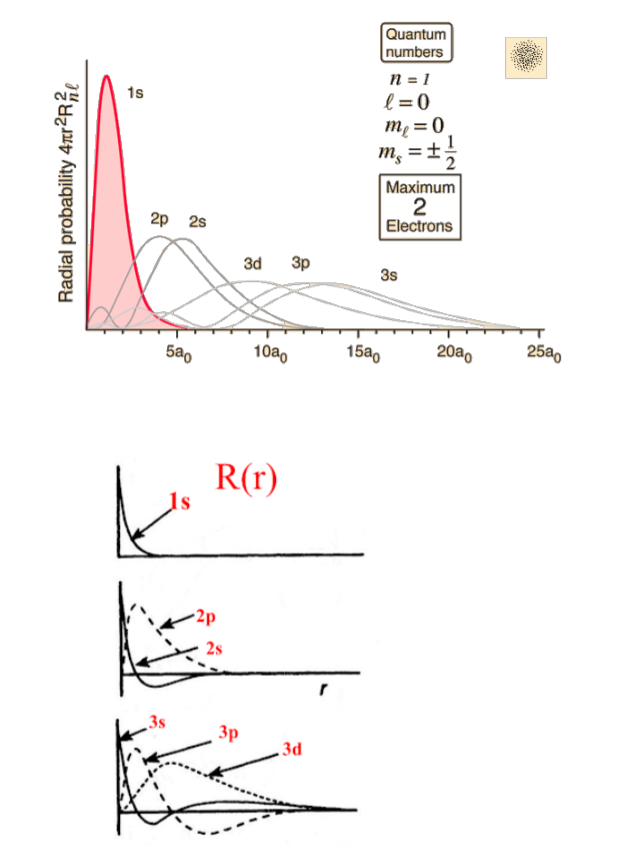
\includegraphics[scale=0.7]{1.png}}

\end{figure}


\par\smallskip
	
Итак, электрон как волна присутствует одновременно на всех
конечных расстояниях от ядра (кроме узлов, при их наличии), но с
разной вероятностью. Иначе говоря, электронная плотность на
разных расстояниях от ядра различна.	

\par\smallskip
	
Очевидно, что площади под графиком любой такой функции равна
единице - ведь это вероятность нахождения электрона на
бесконечности, а мы знаем, что он там точно есть.

\par\smallskip
	
Из графиков следует, что электронная плотность для s-орбиталей
вблизи ядра выше, чем для $p$-, $d$-, и $f$-орбиталей. Говорят, что $s$-орбитали обладают большей проникающей способностью к ядру.	

\par\smallskip
	
Угловая составляющая волновой функции определяет форму
электронного облака орбиталей и их ориентацию в пространстве.
Важно, что с каждым следующим значением главного квантового
числа добавляется одна узловая поверхность, например:

\par\smallskip

\begin{figure}[h]
\centering
 {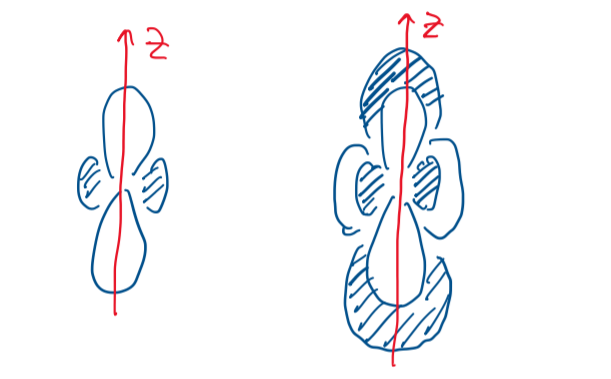
\includegraphics[scale=0.7]{2.png}}
\end{figure}

\par\smallskip


Естественно, что для данной орбитали электрон может находиться
за ее пределами (как по рисунку), мы просто так рисуем, чтобы
добиться некой заданной большой вероятности нахождения
электрона (см. про атомную орбиталь).	

\par\bigskip
\par\bigskip
	